\documentclass[final]{beamer}
\usepackage[scale=1.24]{beamerposter}
\usepackage{graphicx,booktabs,tabularx}
\usepackage{helvet}

\usetheme{confposter}
\setbeamercolor{block title}{fg=Maroon,bg=white}
\setbeamercolor{block body}{fg=black,bg=white}
\setbeamercolor{block alerted title}{fg=white,bg=Maroon!70}
\setbeamercolor{block alerted body}{fg=black,bg=Maroon!10}

\newlength{\sepwid}
\newlength{\onecolwid}
\newlength{\twocolwid}
\newlength{\threecolwid}
\setlength{\paperwidth}{48in}
\setlength{\paperheight}{48in}
\setlength{\sepwid}{0.024\paperwidth}
\setlength{\onecolwid}{0.22\paperwidth}
\setlength{\twocolwid}{0.464\paperwidth}
\setlength{\threecolwid}{0.708\paperwidth}
\setlength{\topmargin}{-0.5in}
\newcolumntype{Y}{>{\centering\arraybackslash}X}


\title{Fido: A Universal Robot Control System Using\\Reinforcement Learning with Limited Feedback}
\author{\LARGE Joshua Gruenstein \and Michael Truell}
\institute{\mbox{}}

\begin{document}

\addtobeamertemplate{block end}{}{\vspace*{2ex}}
\addtobeamertemplate{block alerted end}{}{\vspace*{2ex}}
\setlength{\belowcaptionskip}{2ex}
\setlength\belowdisplayshortskip{2ex}

\begin{frame}[t]
\begin{columns}[t]

\begin{column}{\sepwid}\end{column}
\begin{column}{\onecolwid}

	\begin{alertblock}{Control System Objectives}
		Fido was created to fulfill the following goals:
		\begin{itemize}
			\item \textbf{Trainability}: Allow both human and autonomous training and retraining rather than programming
			\item \textbf{Universality}: Run on any robot and perform any task, even without prior knowledge of the host
			\item \textbf{Speed}: Require few learning iterations and low latency for quick and efficient training
		\end{itemize}
		To achieve this we developed a novel machine learning algorithm utilizing wire-fitted Q-Learning with a neural network, a probabilistic action selection model, and history sampling.  The control system could be trained at a rate \textbf{3 times greater} than the industry standard, allowing practicality over traditional pre-programmed control systems.
	\end{alertblock}

	\begin{block}{System Overview}
		\begin{figure}
			\centering
			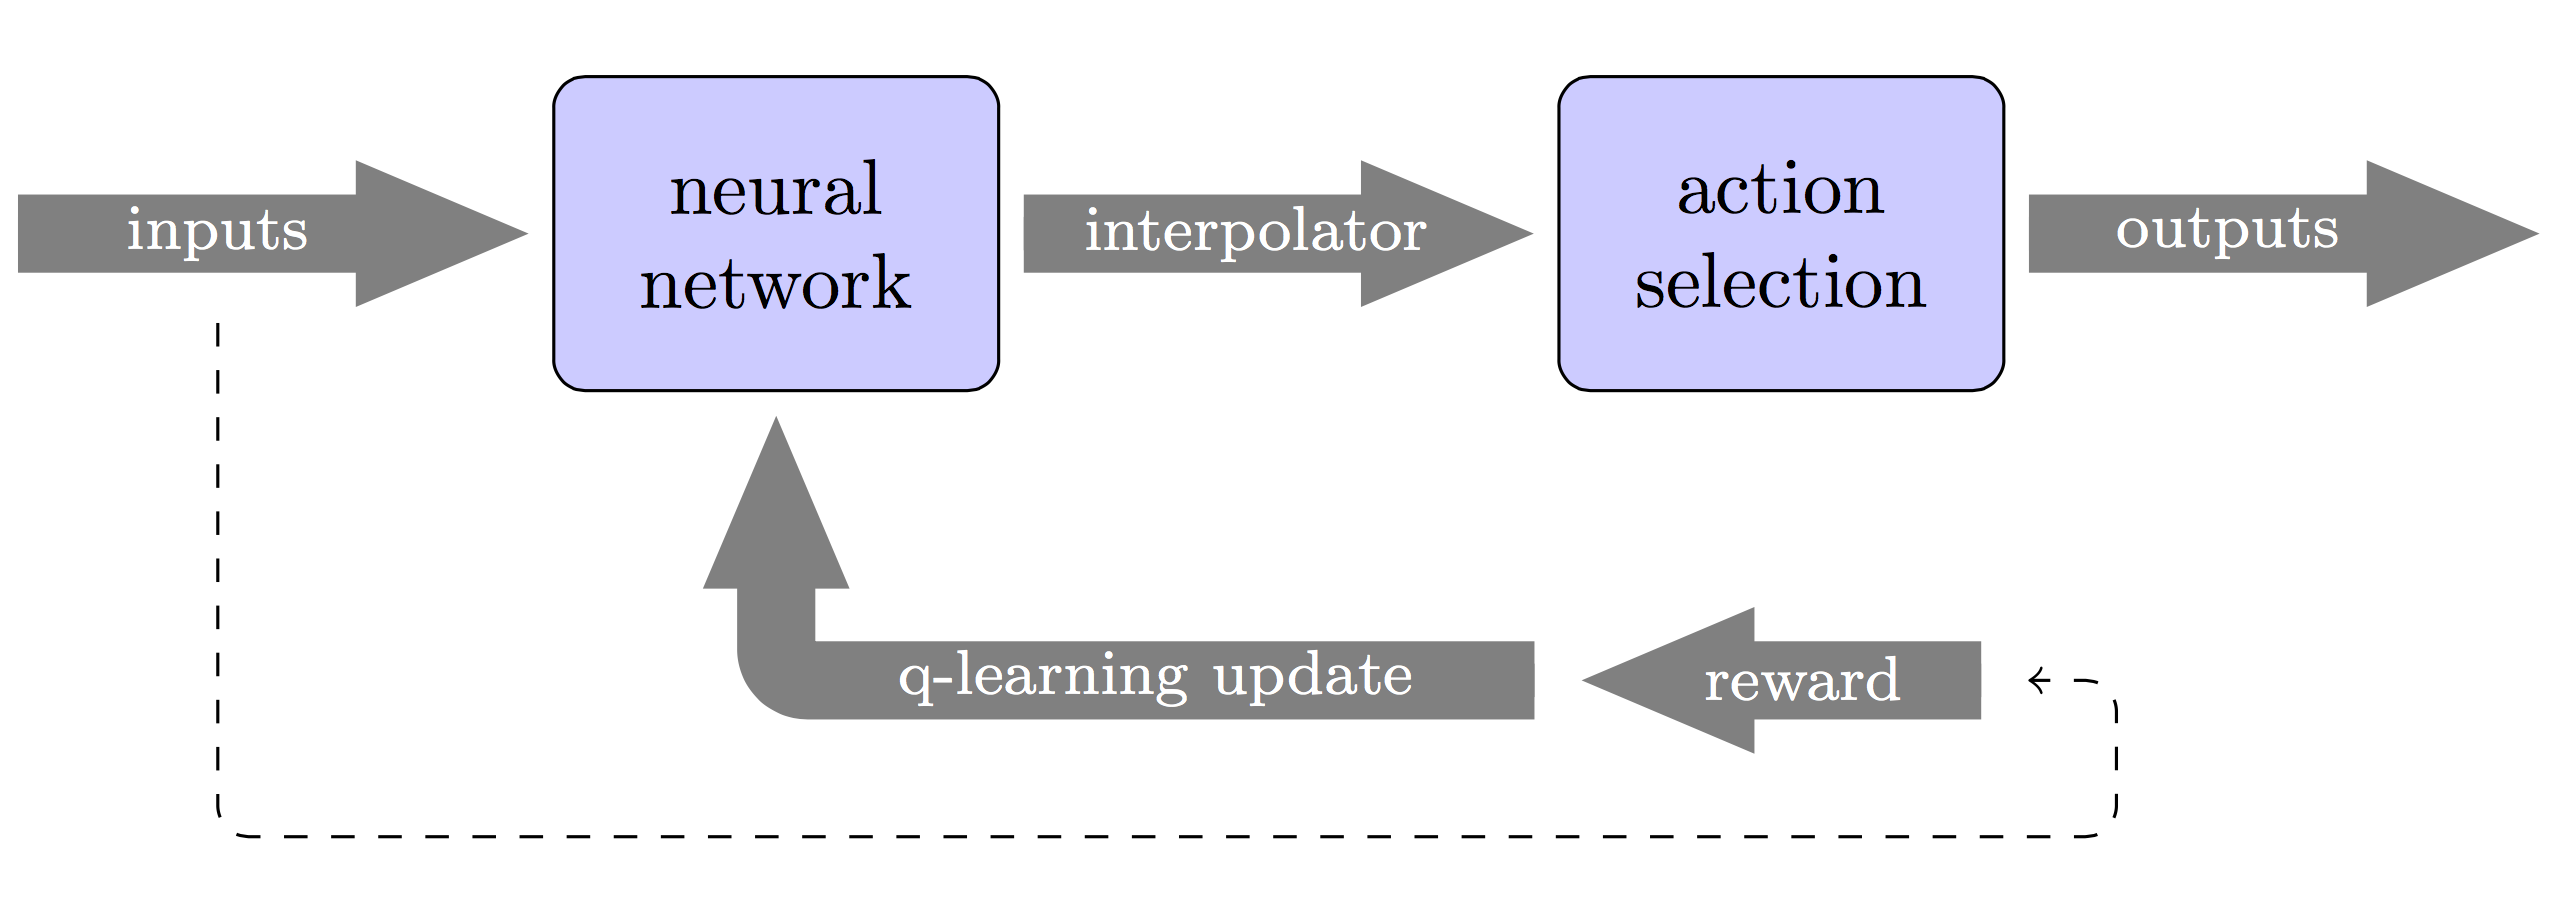
\includegraphics[width=\linewidth]{Figures/diagramRendered.png}
			\caption{Control System Diagram}
		\end{figure}
		\vspace{-1cm}
		\begin{itemize}
			\item From a macro perspective, Fido can be viewed as a ``black box:'' inputs go in and outputs go out, Fido must optimize the relationship of inputs to outputs to maximize reward
			\item  \textbf{Reward system:} Trying to determine the expected reward for an action in a given state based on past reward received
			\begin{itemize}
				\item Must have a scalable, performance-optimized way of storing past state-reward sets and detecting patterns
			\end{itemize}
		\end{itemize}
	\end{block}

\end{column}

\begin{column}{\sepwid}\end{column}

\begin{column}{\twocolwid}

\vspace{-1.65cm}

\begin{columns}[t,totalwidth=\twocolwid]

	\begin{column}{\onecolwid}
		\begin{block}{Reinforcement Learning}
			\begin{itemize}
				\item \textbf{Q-Learning:} Develops a function that intakes a state-action pair and outputs expected utility
				\item Ordinarily, the Q-function is modeled by storing state-action pairs in a table
				\begin{itemize}
					\item Is impractical for large state spaces, use a function approximator instead: \textbf{Artificial Neural Networks}
				\end{itemize}

				\item Usually discrete: no relation made between states or actions

				\begin{itemize}
					\item Can be optimized by coupling a wire-fitted interpolator with our neural network (\textbf{Wire-Fitted Q-Learning})
				\end{itemize}

				\item Cannot just pick the action with the greatest expected utility: must ``explore'' to be trainable and re-trainable
				\begin{itemize}
					\item Use a \textbf{Boltzmann Probability Distribution} selection policy
				\end{itemize}
			\end{itemize}
			\vspace{-1.25cm}
		\end{block}
		\begin{block}{Action Selection}
			\begin{itemize}
				\item Function approximators modeled after nature with the capability to take in a large number of inputs, parallelly process them, and produce a set of outputs
			\end{itemize}
			\vspace{-1.2cm}
			\begin{figure}
				\centering
				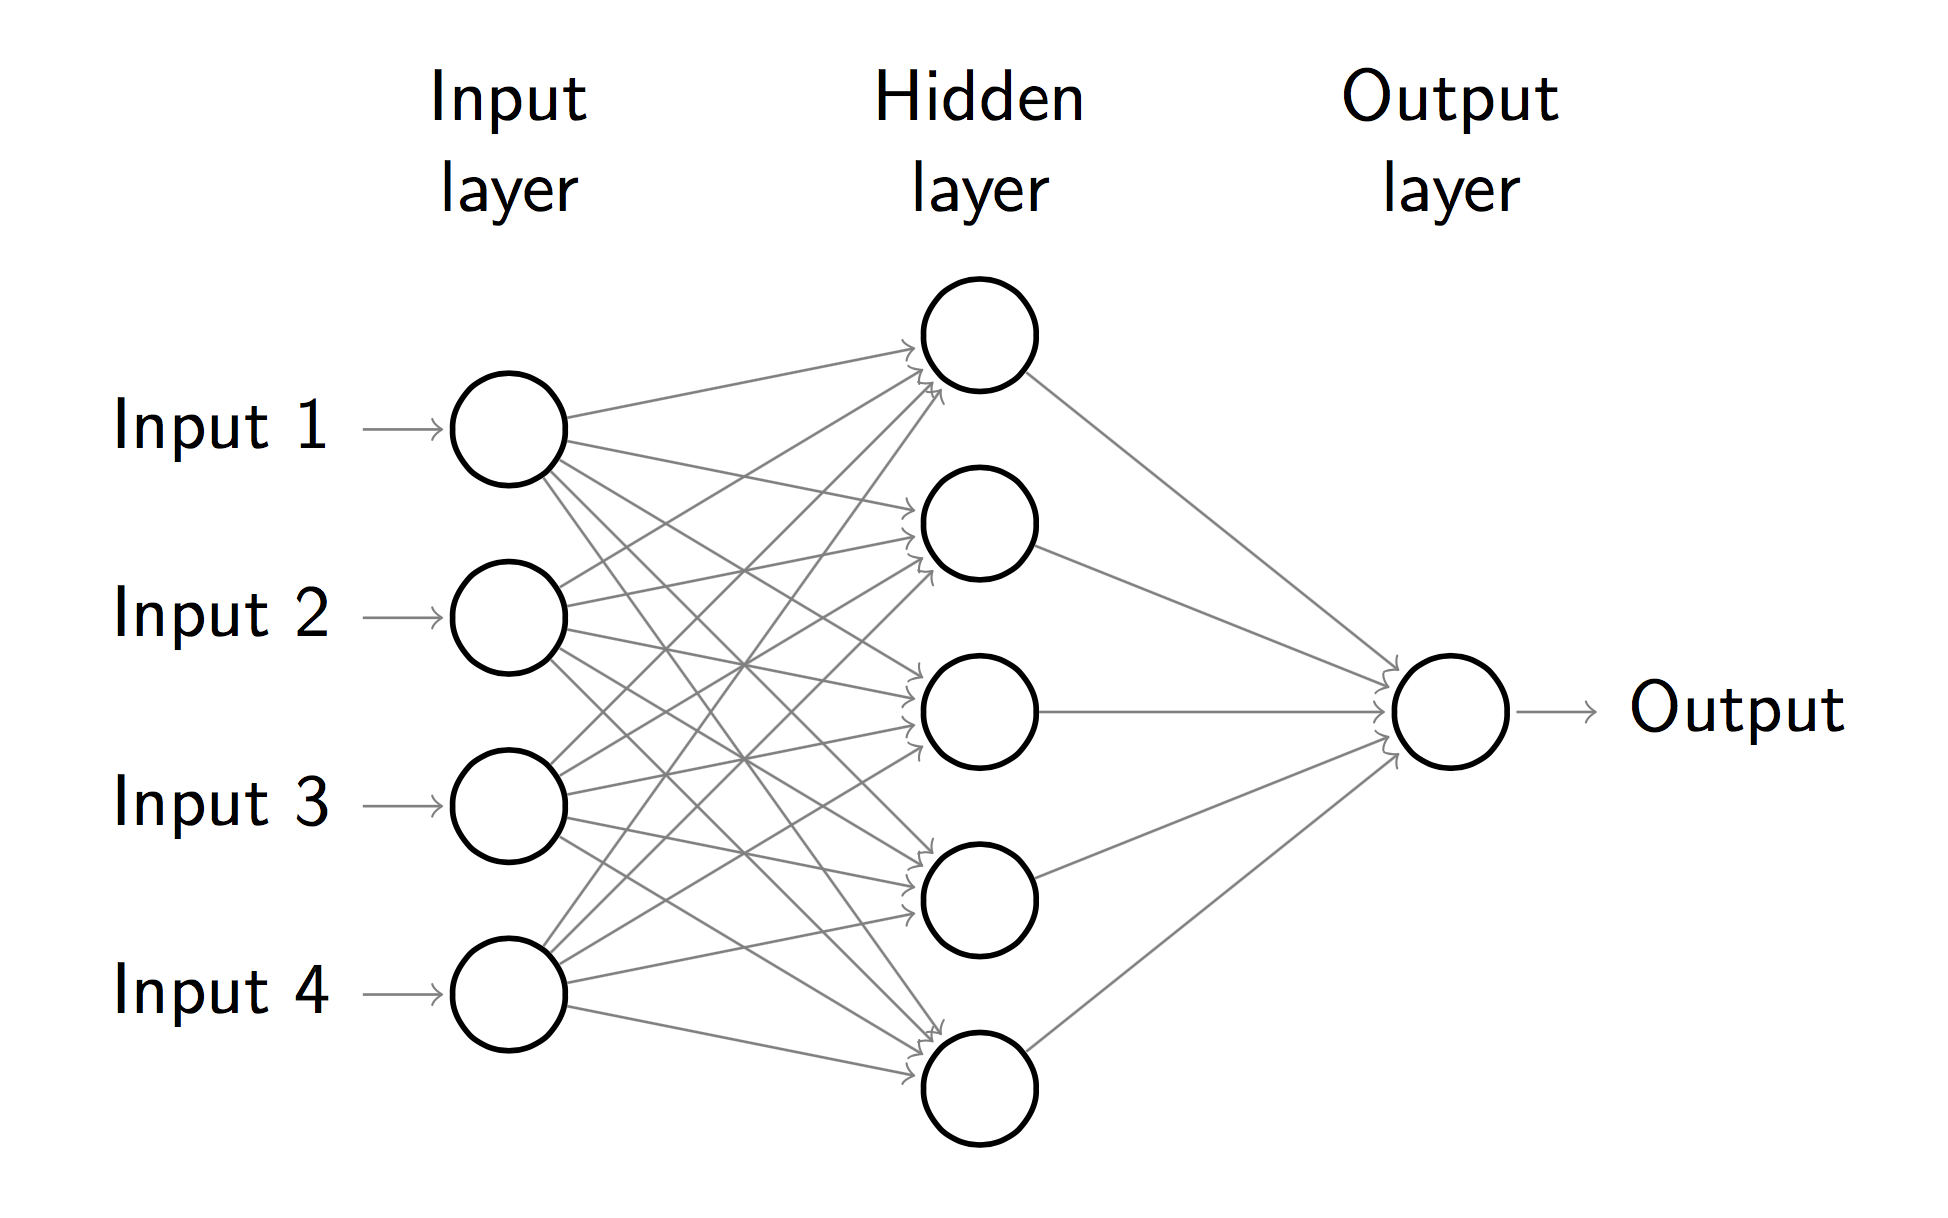
\includegraphics[width=.8\linewidth]{Figures/FeedForwardRendered}
				\caption{Single Output Feed-forward Neural Network}
				\label{fig:feedforward}
			\end{figure}
			\vspace{-3cm}
		\end{block}
	\end{column}

	\begin{column}{\onecolwid}\begin{block}{Training}


	\begin{itemize}
		\item \textbf{Neural Networks:} Function approximators modeled after nature with the capability to take in a large number of inputs, parallelly process them, and produce a set of outputs
	\end{itemize}
	
	\begin{figure}
		\centering
		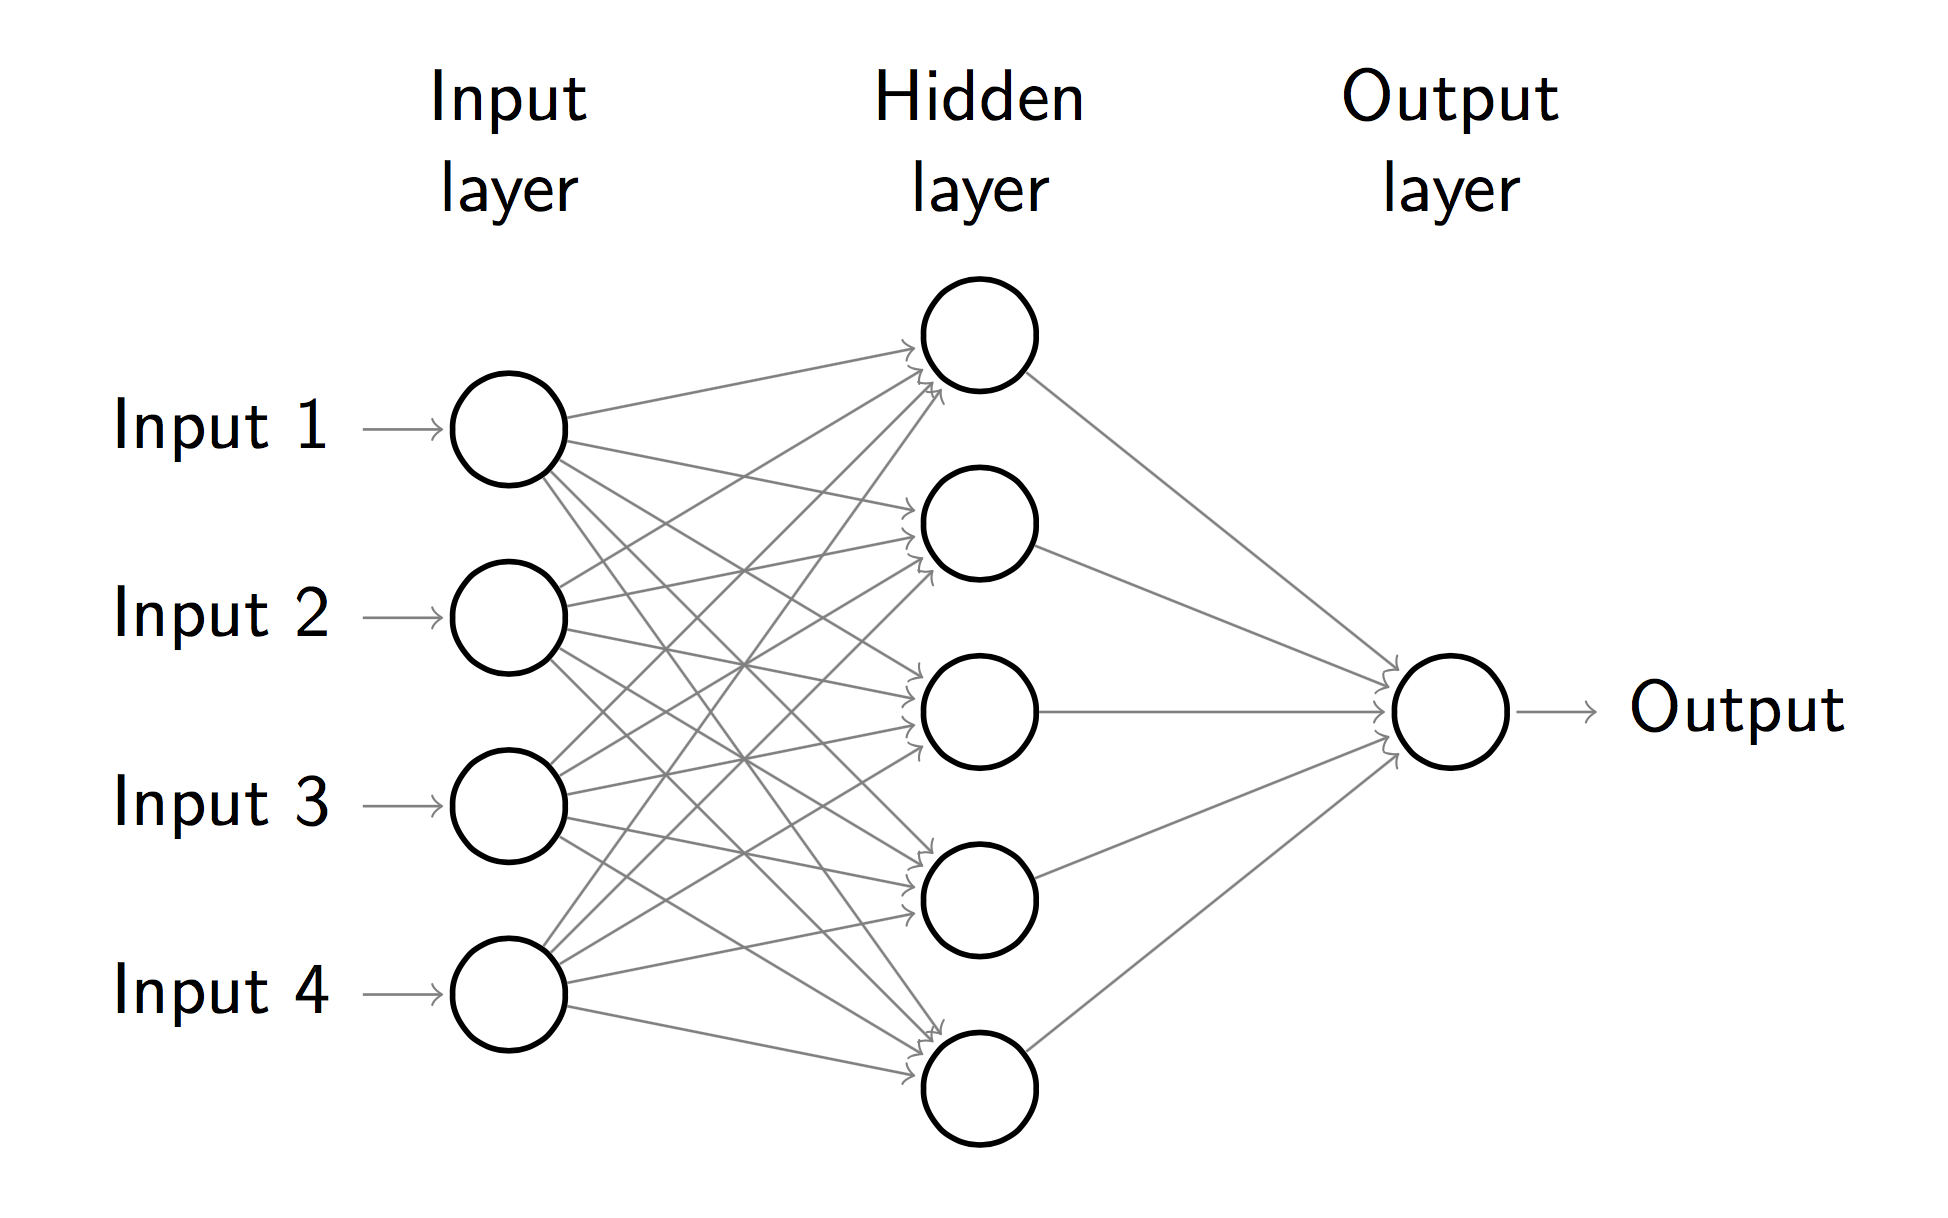
\includegraphics[width=.8\linewidth]{Figures/FeedForwardRendered}
		\caption{Single Output Feed-forward Neural Network}
		\label{fig:feedforward}
	\end{figure}

	\begin{itemize}
		\item \textbf{History Sampling:} Develops a function that intakes a state-action pair and outputs expected utility
		\item Ordinarily, the Q-function is modeled by storing state-action pairs in a table
		\begin{itemize}
			\item Is impractical for large state spaces, use a function approximator instead: \textbf{Artificial Neural Networks}
		\end{itemize}

		\item Usually discrete: no relation made between states or actions

		\begin{itemize}
			\item Can be optimized by coupling a wire-fitted interpolator with our neural network (\textbf{Wire-Fitted Q-Learning})
		\end{itemize}

		\item Cannot just pick the action with the greatest expected utility: must ``explore'' to be trainable and re-trainable
		\begin{itemize}
			\item Use a \textbf{Boltzmann Probability Distribution} selection policy
		\end{itemize}
	\end{itemize}

\end{block}\end{column}

\end{columns}


	\begin{block}{Results}
		Results were gathered both from simulation and hardware for a variety of tasks.  Gathered data for each task included the number of learning iterations, or how many pieces of reward it took for Fido to master the task, action selection time, or the latency in probabalistic action selection, and training time, or the latency in updating Fido's model.
		\begin{table}[ht]
			\centering
			\caption {Fido Results in Simulation} \label{tab:simresults}
			\begin{tabularx}{.9\textwidth}{l||Y|Y|Y}
				\toprule
				Task        & Learning Iterations & Action Selection (ms) & Training Time (ms) \\ \midrule
				Flash       & 6                   & 0.                  & 6               \\
				Float to Point       & 14                  & 1                  & 6               \\
				Drive to Point       & 17                  & 1                  & 11              \\
				Line Following       & 18                                    & 0.               & 2               \\
				Noisy Line Following       & 21                                   & 0.               & 105               \\
				\bottomrule
			\end{tabularx}
		\end{table}
		\vspace{.5cm}

		\begin{table}[ht]
			\centering
			\caption {Fido Results on Thing One} \label{tab:thingoneresults}
			\begin{tabularx}{.9\textwidth}{l||Y|Y|Y}
				\toprule
				Task              & Learning Iterations & Action Selection (ms) & Training Time (ms) \\ \midrule
				Stay Still        & 3                   & 1                    & 43.5                  \\
				Drive to Point    & 18                  & 4                     & 65                  \\
				\bottomrule
			\end{tabularx}
		\end{table}

		\begin{table}[ht]
			\centering
			\caption {Fido Results on Thing Two} \label{tab:thingtworesults}
			\begin{tabularx}{.9\textwidth}{l||Y|Y|Y}
				\toprule
				Task              & Learning Iterations & Action Selection (ms) & Training Time (ms) \\ \midrule
				Drive Straight         & 13                   & 2                    & 30                 \\
				Line Following         & 15                  & 21                    & 95                \\
				Fetch                  & 8                  & 1                     & 70                 \\
				Limping Line Following & 6                   & 20                    & 37                 \\
				\bottomrule
			\end{tabularx}
		\end{table}

	\end{block}

\end{column}

\begin{column}{\sepwid}\end{column}

\begin{column}{\onecolwid}
	\begin{block}{Implementation}
		Fido was programmed in C++, with no external dependencies.  However, the simulator does use the SFML graphics library.  The hardware implementation uses the Intel Edison embedded platform, a 3D printed chassis and a differential drive system.

		\begin{figure}
			\centering
			\fbox{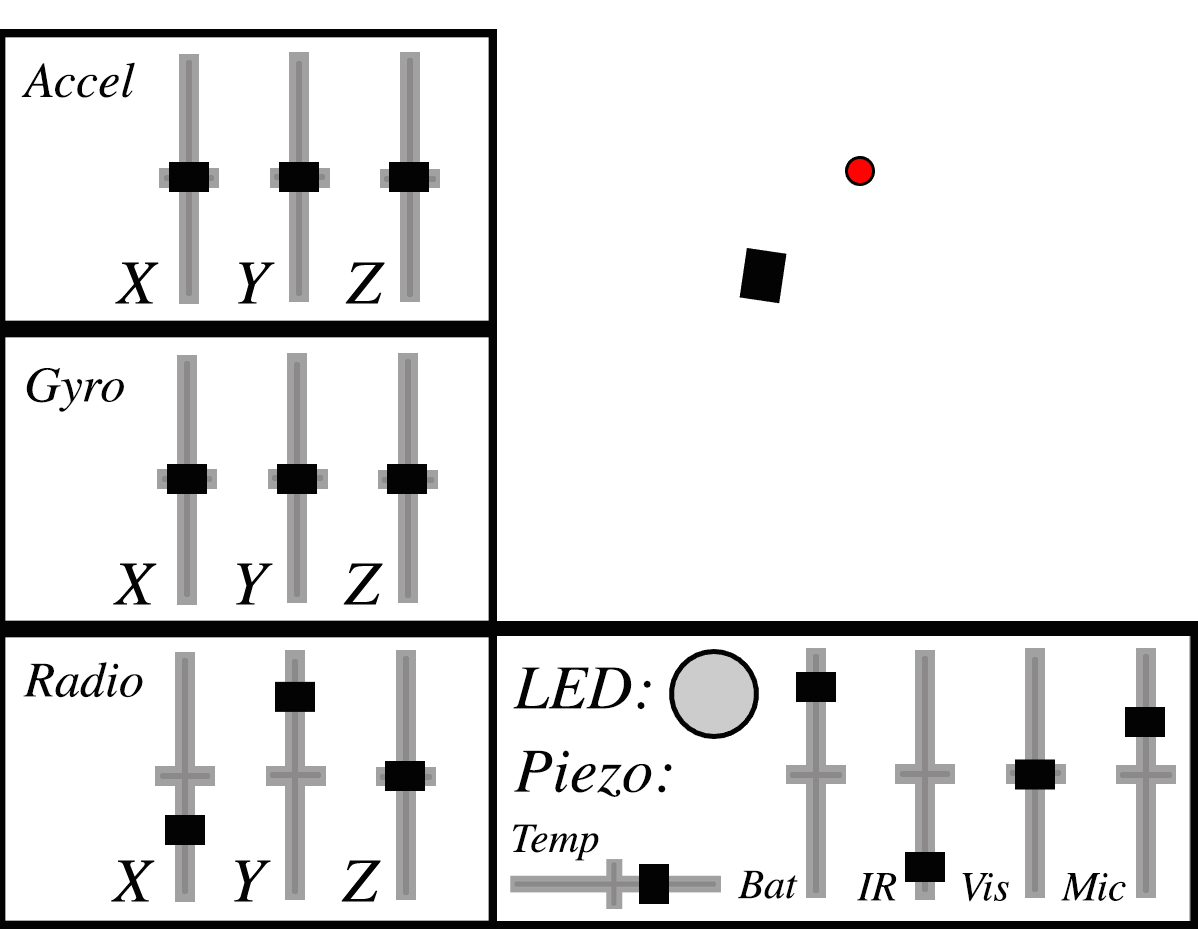
\includegraphics[width=.75\linewidth]{Figures/Screenshot.png}}
			\caption{Fido Simulator Graphical User Interface}
		\end{figure}
	\end{block}

	\begin{block}{Applications}
		We would like to experiment with dynamic optimization of hyperparameters, changing factors such as neural network architecture and Boltzman temperature constant to best fit the task at hand.  We also plan to package Fido as a machine learning library for embedded electronics and robotics, and build a microcontroller-based hardware implementation to further explore for resource-limited environments.
	\end{block}

	\begin{block}{Selected References}
		\nocite{*}
		{\fontsize{25}{30}\bibliographystyle{IEEEtran}\bibliography{Poster}\vspace{0.75in}}
	\end{block}

\end{column}

\end{columns}
\end{frame}
\end{document}

%%%%%%%%%%%%%%%%%%%%%%%%%%%%%%%%%%%%%%%%%
% Adapted from "Jacobs Landscape Poster"
% https://teamwork.jacobs-university.de:8443/confluence/display/CoPandBiG/LaTeX+Poster
% License: CC BY-NC-SA 3.0 (http://creativecommons.org/licenses/by-nc-sa/3.0/)
%%%%%%%%%%%%%%%%%%%%%%%%%%%%%%%%%%%%%%%%%
